\documentclass{article}
\usepackage{tikz}
\usetikzlibrary{intersections}
\usetikzlibrary{arrows, arrows.meta}
\tikzset{help lines/.style=very thin}
\tikzset{Karl's grid/.style={help lines, color=#1!50},
         Karl's grid/.default=blue}
\begin{document}
We are working on
  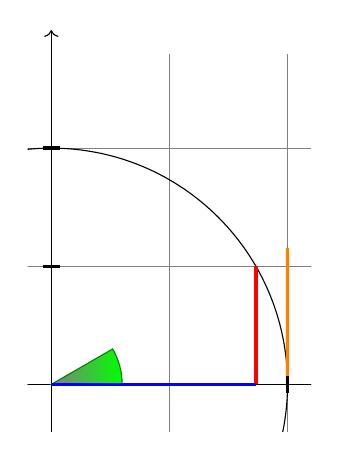
\begin{tikzpicture}[scale=3]
    %\draw[Karl's grid=red] (0,0) grid (5,5);
    \clip (-0.1,-0.2) rectangle (1.1, 1.51);
    \draw[step=0.5cm, gray, very thin] (-1.4,-1.4) grid (1.4,1.4);
    \draw[->] (-1.5,0)--(1.5,0);
    \draw[->] (0,-1.5)--(0,1.5); %Now add the half circle
    \draw (0,0) circle [radius=1cm];
    \shadedraw[left color=gray,right color=green,draw=green!50!black] (0,0)--(3mm,0mm)
      arc [start angle=0, end angle=30, radius=3mm]--cycle;
    % \filldraw[fill=green!20!white, draw=green!50!black] (0,0)--(3mm,0mm)
    %   arc [start angle=0, end angle=30, radius=3mm]--cycle;
    \draw[red, very thick] (30:1cm) -- +(0,-0.5);
    \draw[blue, very thick] (30:1cm) ++(0,-0.5) -- (0,0);
    \path [name path=upward line] (1,0) -- (1,1);
    \path [name path=sloped line] (0,0) -- (30:1.5cm);
    \draw [name intersections={of=upward line and sloped line, by=x}]
      [very thick, orange] (1,0) -- (x);
    %\draw[red, very thick] (30:1cm)--(30:1cm |- 0,0)--(0,0);

    \foreach \x in {-1cm, -0.5cm, 1cm}
      \draw[very thick] (\x,-1pt)--(\x,1pt);
    \foreach \y in {-1cm, -0.5cm, 0.5cm, 1cm}
      \draw[very thick] (-1pt,\y)--(1pt,\y);
    % \foreach \x in {-1, -0.5, 1}
    %   \draw[xshift=\x cm] (0pt,-1pt)--(0pt,1pt);
  \end{tikzpicture}
% scrap drawing
Curved Path Construction.
  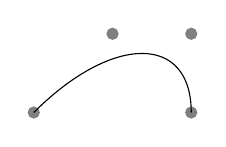
\begin{tikzpicture}
    \filldraw[gray] (0,0) circle [radius=2pt]
                    (1,1) circle [radius=2pt]
                    (2,1) circle [radius=2pt]
                    (2,0) circle [radius=2pt];
    \draw (0,0) .. controls (1,1) and (2,1) .. (2,0);
  \end{tikzpicture}
  \tikz \draw (0,0) circle [radius=10pt];
  \tikz \draw[rotate=30] (0,0) ellipse [x radius=20pt,y radius=10pt];
  \tikz \draw[x=1.57ex,y=1ex] (0,0) sin (1,1) cos (2,0) sin (3,-1) cos (4,0)
                              (0,1) cos (1,0) sin (2,-1) cos (3,0) sin (4,1);
  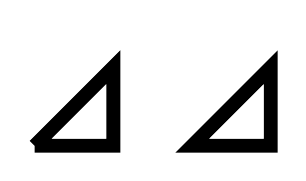
\begin{tikzpicture}[line width=5pt]
    \draw (0,0) -- (1,0) -- (1,1) -- (0,0);
    \draw (2,0) -- (3,0) -- (3,1) -- cycle;
    \useasboundingbox (0,1.5); %make bounding box higher.
  \end{tikzpicture}
  \tikz \shade (0,0) rectangle (2,1) (3,0.5) circle (.5cm);
  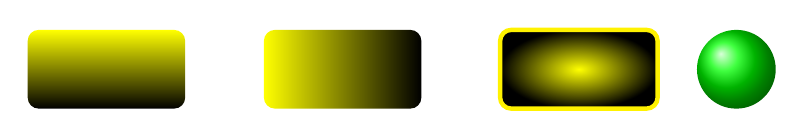
\begin{tikzpicture}[rounded corners, ultra thick]
    \shade[top color=yellow, bottom color=black] (0,0) rectangle +(2,1);
    \shade[left color=yellow, right color=black] (3,0) rectangle +(2,1);
    \shadedraw[inner color=yellow, outer color=black, draw=yellow] (6,0) rectangle +(2,1);
    \shade [ball color=green] (9,0.5) circle (.5cm);
  \end{tikzpicture}
  % difference between + and ++
  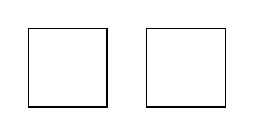
\begin{tikzpicture}
    \def \rectanglepath{-- ++(1cm,0cm)-- ++(0cm,1cm)-- ++(-1cm,0cm)-- cycle}
    \draw (0,0) \rectanglepath;
    \draw (1.5,0) \rectanglepath;
  \end{tikzpicture}
  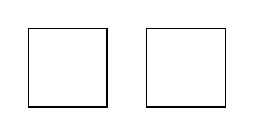
\begin{tikzpicture}
    \def \rectanglepath{-- +(1cm,0cm) -- +(1cm,1cm) -- +(0cm,1cm) -- cycle}
    \draw (0,0) \rectanglepath;
    \draw (1.5,0) \rectanglepath;
  \end{tikzpicture}
  \tikz \draw (0,0) rectangle +(1,1) (1.5,0) rectangle +(1,1);
  % arrow
  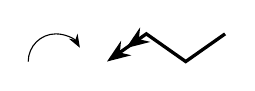
\begin{tikzpicture}[>=Stealth]
    \draw[->] (0,0) arc [start angle=180, end angle=30, radius=10pt];
    \draw[<<-,very thick] (1,0) -- (1.5cm,10pt) -- (2cm,0pt) -- (2.5cm,10pt);
  \end{tikzpicture}
  $?$ Scoping has another interesting effect: Any changes to the clipping area are local to
  the scope. Thus, if you say \verb+\clip+ somewhere inside a scope, the effect of the \verb+\clip+
  command ends after the end of that scope.
  \tikz \draw (0,0) -- (0,0.5) [xshift=2pt] (0,0) -- (0,0.5);
  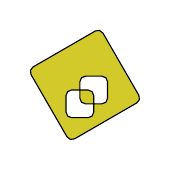
\begin{tikzpicture}[even odd rule, rounded corners=2pt, x=10pt, y=10pt]
    \filldraw[fill=yellow!80!black] (0,0) rectangle (1,1)
          [xshift=5pt, yshift=5pt]  (0,0) rectangle (1,1)
          [rotate=30]             (-1,-1) rectangle (2,2);
  \end{tikzpicture}
  \foreach \x in {1,2,3} {$x=\x$, }
%Venn diagram, Till Tantau
\def\firstcircle{(0,0) circle (1.5cm)}
\def\secondcircle{(45:2cm) circle (1.5cm)}
\def\thirdcircle{(0:2cm) circle (1.5cm)}

% Now we can draw the sets:
\begin{tikzpicture}

    \begin{scope}[even odd rule]
      \clip \secondcircle;
      \clip \firstcircle;
      \clip \thirdcircle (-3,-3) rectangle (3,3);
      \fill[red] \secondcircle;
    \end{scope}
    \draw \firstcircle node[below] {$A$};
    \draw \secondcircle node [above] {$B$};
    \draw \thirdcircle node[below] {$C$};
\end{tikzpicture}
%End of the Venn diagram.
% Drawing a series of circles using TikZ
\tikz \foreach \x in {1,...,10}
        \draw (\x,0) circle [radius=0.4cm];
We can also nest loops to create interesting effects.
\end{document}
